\Chapter{Dataset: Duke Breast Cancer MRI}

\Section{Composizione del Dataset}

Il dataset utilizzato proviene dal database \textbf{Duke Breast Cancer MRI} \cite{duke_breast_mri}, un archivio pubblico messo a disposizione dalla \textbf{Duke University Medical Center} e accessibile tramite il portale \textbf{The Cancer Imaging Archive (TCIA)}. Questo dataset è stato sviluppato per promuovere la ricerca nel campo della segmentazione automatica della mammella e contiene immagini di \textbf{risonanza magnetica (MRI)} acquisite da pazienti con diagnosi confermata di carcinoma mammario invasivo.

Ogni studio è composto da sequenze MRI in formato \textbf{DICOM}, ottenute in posizione prona utilizzando scanner da \textbf{1.5 T} o \textbf{3.0 T} (\textbf{prodotti da GE Healthcare o Siemens}). Le immagini sono acquisite in \textbf{proiezione assiale}, con una \textbf{risoluzione spaziale variabile} compresa tra \textbf{0.6×0.6×1.0 mm\textsuperscript{3}} e \textbf{1.1×1.1×1.2 mm\textsuperscript{3}}, rendendole adatte all'elaborazione tridimensionale.

\begin{wrapfigure}{r}{0.4\textwidth} 
  	\centering 
 	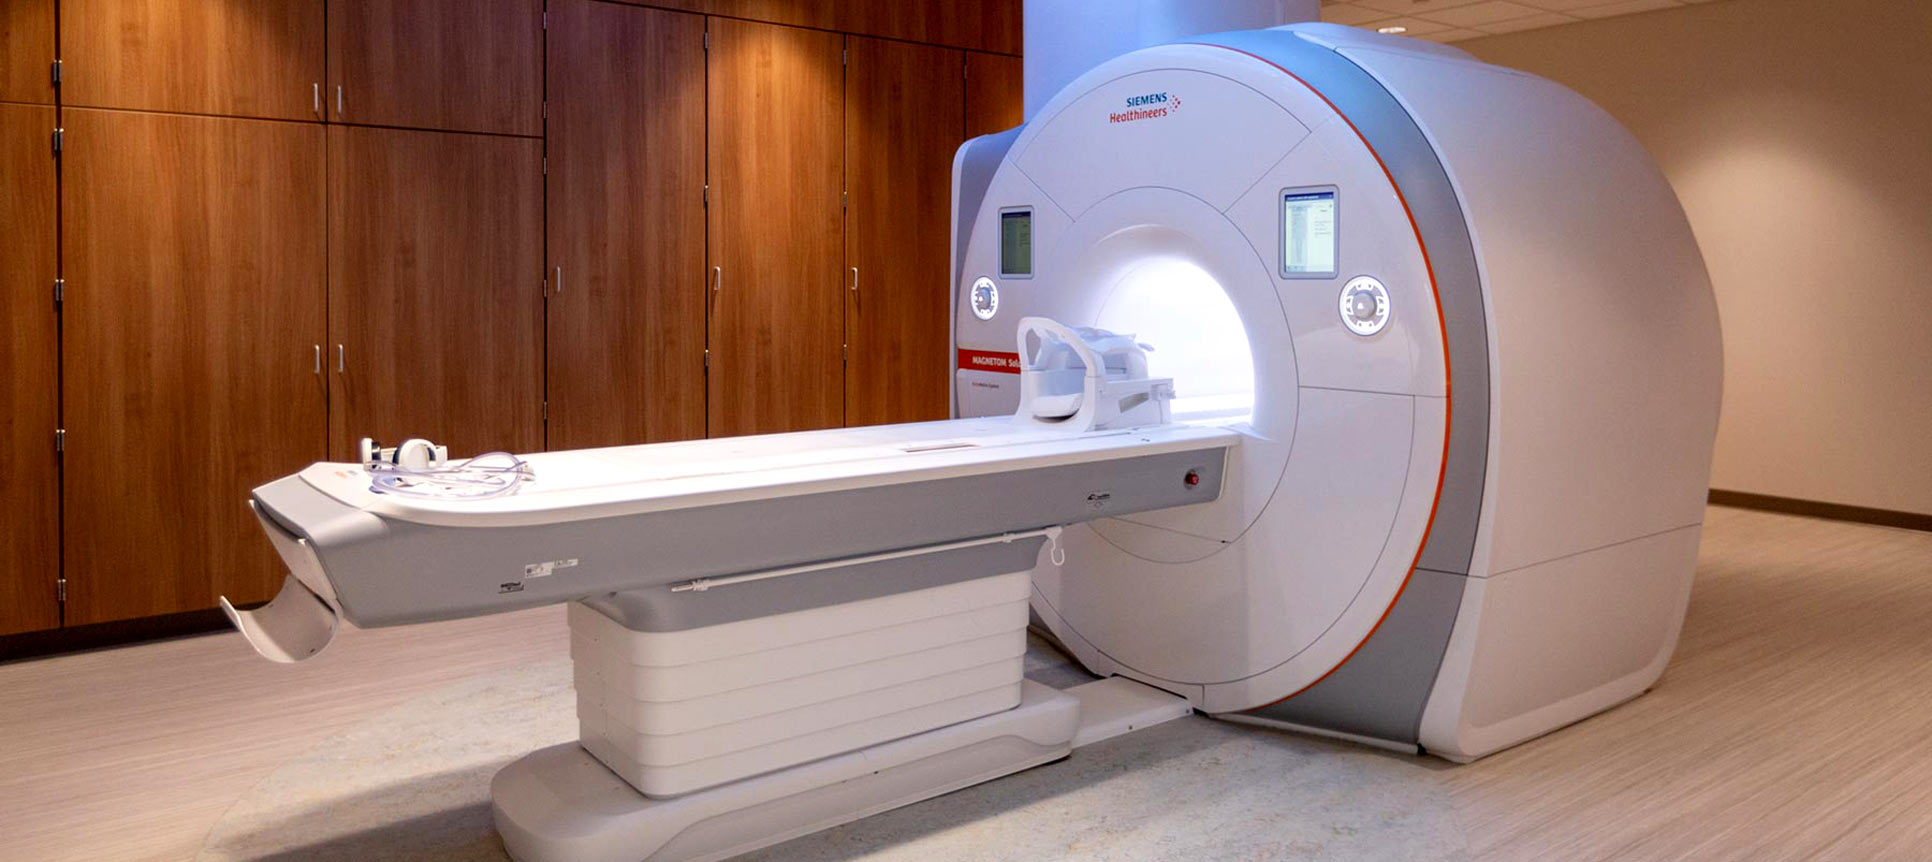
\includegraphics[width=0.4\textwidth]{images/2025-08-09-19-34-01.png} 
    \caption{Fast Breast MRI Available to Women with Average Breast Cancer Risk | Duke Health \cite{mri_machine}}
 \end{wrapfigure} 


Le sequenze utilizzate nel progetto corrispondono alle immagini \textbf{T1-weighted fat-suppressed pre-contrast}, selezionate per l’elevato contrasto tra il \textbf{tessuto adiposo} e quello \textbf{fibroghiandolare (FGT),} senza l’interferenza di mezzi di contrasto. Questa scelta metodologica è coerente con quanto proposto da \textbf{Lew et al. (2024),} che hanno dimostrato l’efficacia di tale sequenza per la segmentazione automatica del FGT e dei vasi sanguigni.

\Subsection{Annotazioni e Ground Truth}
Una caratteristica distintiva del dataset è la disponibilità di \textbf{annotazioni manuali tridimensionali}, elaborate da \textbf{annotatori formati} e successivamente validate da \textbf{radiologi esperti in senologia}. Ogni caso include \textbf{segmentazioni voxel-wise} delle seguenti strutture:
\begin{itemize}
\item \textbf{Seno (breast)}: delimitazione del tessuto mammario escludendo parete toracica, sternale e linfonodi;
\item \textbf{Tessuto fibroghiandolare (FGT)}: zone a maggiore densità che costituiscono l’indicatore primario per la valutazione del rischio;
\item \textbf{Vasi sanguigni}: rami dell’arteria mammaria interna e dell’arteria toracica laterale, spesso iperintensi anche in assenza di contrasto.
\end{itemize}


\Subsection{Preprocessing e Integrazione con MONAI}
Durante la fase di preparazione, le immagini DICOM sono state convertite in un formato compatibile con \textbf{MONAI (Medical Open Network for AI)} \cite{cardoso2022monai}.



La pipeline di preprocessing ha incluso le seguenti operazioni:
\begin{itemize}
\item il \textbf{caricamento} delle immagini e delle relative maschere;
\item la \textbf{normalizzazione} dell’intensità per migliorare la stabilità del training;
\item il \textbf{ridimensionamento} delle immagini a una risoluzione uniforme per l’input nei modelli di rete neurale;
\item la conversione in \textbf{dizionari Python} contenenti l'immagine e la maschera;
\item il \textbf{salvataggio} del dataset preprocessato su disco, pronto per essere utilizzato nel training.
\end{itemize}


\Subsection{Suddivisione del Dataset}

\begin{wrapfigure}{r}{0.4\textwidth} 
  	\centering 
 	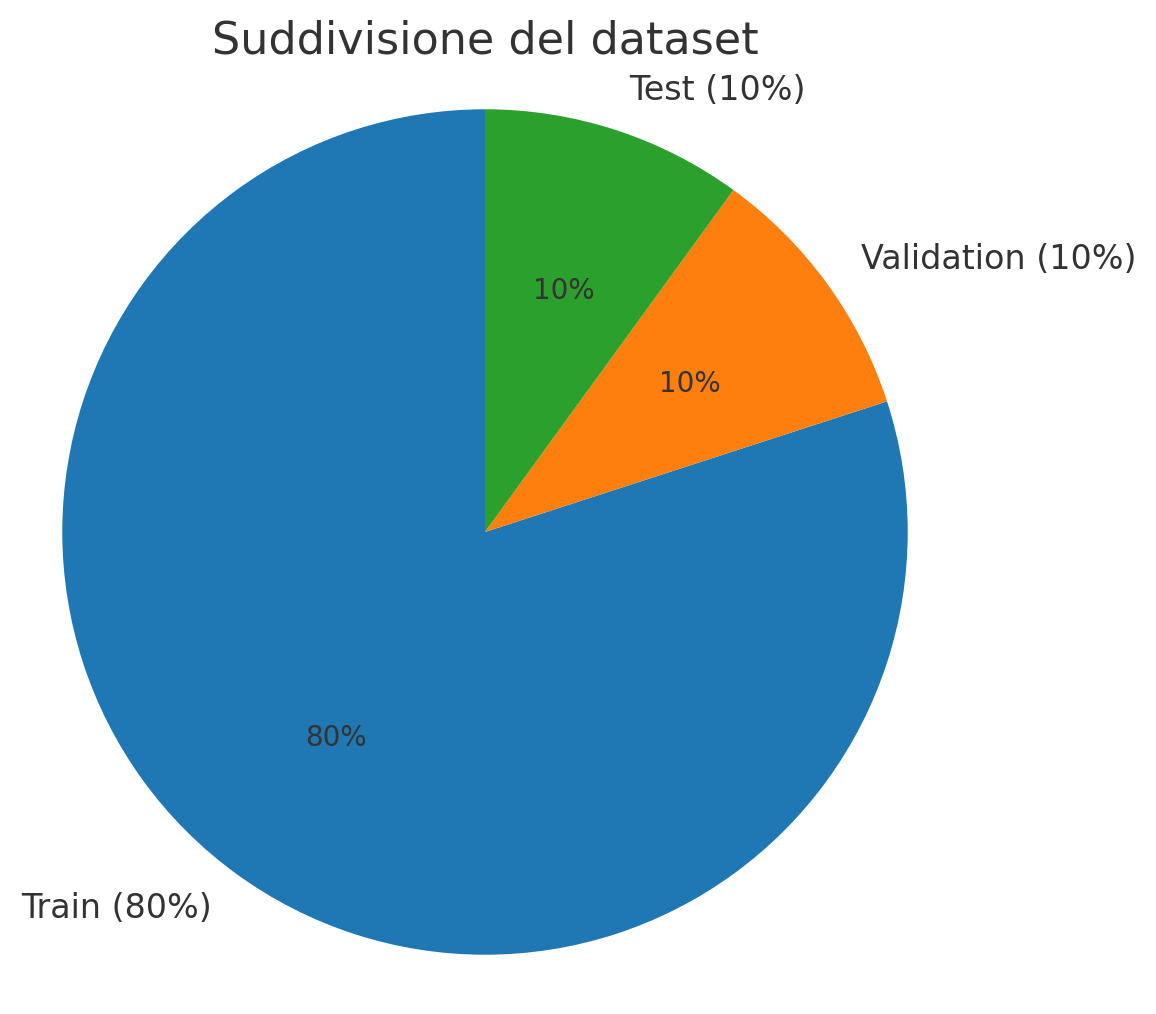
\includegraphics[width=0.4\textwidth]{figures/split_pie_chart.png} 
    \caption{Grafico a torta della suddivisione del dataset}
 \end{wrapfigure} 

Al fine di garantire una valutazione robusta e riproducibile dei modelli, l'intero dataset è stato suddiviso in tre sottoinsiemi:
\begin{itemize}
\item \textbf{Training set} \hlight{(80\%)}: utilizzato per l'addestramento del modello, comprendente la maggior parte dei dati e delle variabilità cliniche;
\item \textbf{Validation set} \hlight{(10\%)}: impiegato durante l’addestramento per monitorare l’overfitting e ottimizzare gli iperparametri;
\item \textbf{Test set} \hlight{(10\%)}: utilizzato esclusivamente per la valutazione finale delle prestazioni del modello, senza interferenze in fase di sviluppo.
\end{itemize}



